\documentclass[8 pt, leqno]{article}
\usepackage[english]{babel}
\usepackage[utf8]{inputenc}
\usepackage{fancyhdr}
\usepackage{wrapfig}
\usepackage[margin=.75in]{geometry}
\usepackage{amssymb,amsmath,amsthm,mathrsfs}
\usepackage{graphicx}
\usepackage{caption}
\usepackage{pgfplots}
\usepackage[utf8]{inputenc}
\usepackage[T1]{fontenc}
\pgfplotsset{
  compat=1.9,
  unit code/.code 2 args={\si{#1#2}} % from manual, for using siunitx to typeset units
}
\usepackage{mdframed}
\usepackage{inputenc}
\usepackage{siunitx}
\usepackage{siunitx}
\usepgfplotslibrary{groupplots,units}
\newlength\figureheight 
\newlength\figurewidth 
\setlength\figureheight{0.4\textwidth}
\setlength\figurewidth{0.35\textwidth}
\usepackage{tikz}
\setcounter{section}{2}
\usepackage[hidelinks]{hyperref}
\usepackage{graphicx}
\usepackage{subcaption}
\usepackage{multicol}




 
\pagestyle{fancy}
\fancyhf{A Novel Approach to Modeling Complex Systems Through Brownian Motion}
    \rhead{}
\lhead{}
\linespread{1.5}

%\title{}
%\date{}
%\author{}
\begin{document}
%\maketitle

Modeling complex systems, from the growth of cancer cells and bacteria to the evolution of a species, is critical to our understanding of the physical world and our place in it. To comprehend our origins, it is essential to accurately model the dynamics driving the creation of life, and to comprehend our future, it is essential to have accurate predictive models. Such modeling is complicated when the dynamics behind these complex systems is random, or stochastic.\\
\indent Current models describing biological processes are deterministic, meaning they do not accurately reflect the randomness of complex systems over long periods of time. Dr. Motsch, a professor of applied biology and statistics in the School of Mathematical and Statistical Sciences, and I will study the same complex systems with the use of Brownian motion in order to obtain more accurate predictions of the behavior of stochastic complex systems. Brownian motion, originally studied by the botanist Robert Brown in the 19th century and popularized by Einstein in the early 20th century, describes motion that behaves stochastically. For instance, if a particle suspended in water were acted upon randomly by other particles, its behavior would be described as Brownian. My research with Dr. Motsch will seek to demonstrate that Brownian motion will accurately model stochastically complex systems and allow us to invent frameworks that derive meaningful insights into the future.\\
\indent In order to quantify the accuracy of our approach, we will be using a tool in mathematics called the Wasserstein Distance, which quantifies the distance between functions or data sets, and thereby provides us insight into the improvement that our approach to modeling stochastic systems offers. We aim to collaborate with
Dr. Pedro Lowenstein, a professor of Neurosurgery at the University of Michigan to obtain data on cancer growth in a mouse, and with this data, we will use the Wasserstein Distance to compute the distance between the true biological data, the predictions made by the Brownian motion approach, and the predictions made by the deterministic approach. We seek to understand how the number of particles used in the Brownian motion approach affects the accuracy of our approximation of the biological data. More specifically, we will propose an algorithm that will determine the number of particles necessary to get within a desired error using the Brownian motion approach. \\
\indent During a summer research project, completed under Dr. Anne Gelb in 2014, I studied the use of statistical algorithms to improve Fourier edge detection in the presence of corrupted data. Specifically, Dr. Gelb and I derived an algorithm for reconstructing MRI images that is 166$\%$ more accurate than previous methods available to the medical community. By working with Dr. Gelb, I developed an interest in using statistical tools to study relevant problems in biology. During the summer of 2016 I participated in two summer research programs that provided me with the interest and background necessary to successfully complete my Origins Project research. My first project was at the University of California, Santa Barbara where I took a series of courses on differential equations in random media, biological modeling of living systems, and statistical approximations of biological processes. Through conversations with professors and graduate students from Princeton, Stanford, UC Berkeley and others, I learned about cutting-edge research at the intersection of biology and statistics and will apply these techniques in my Origins Project research.\\
\indent In my second project, I was selected as one of three from over 300 undergraduates to participate in a research experience at San Diego State University. There I studied the convergence behavior of statistical algorithms used in linear regression models. Specifically, my advisor and I proposed the first algorithm for concrete convergence bounds for the error of a Gibbs sampler in a Bayesian linear regression model. These results will be submitted for publication in October. This research experience taught me the tools to complete statistical convergence analysis, and I will use similar tools to study the convergence behavior of the approximation to complex systems using Brownian motion. \\
\indent To successfully complete this research, I will need an advanced grasp of real analysis, probability theory, and numerical analysis. . I have taken a course on numerical methods with Dr. Motsch, and I have enrolled in graduate courses in real analysis, distribution theory, and stochastic processes. In these courses I will obtain the tools necessary to analyze papers relating to my work with Dr Motsch, as well as make meaningful contributions to the field. In the Spring I will finish the graduate sequence in real analysis and probability theory, creating a solid theoretical foundation that I will use in my research.\\
\indent Developing accurate statistical algorithms for understanding stochastic complex systems is one of the largest problems in modern biological sciences, and the opportunity to study this type of problem has been my main focus during my undergraduate career. In addition to contributing to the field of computational biology, I hope to motivate theoretical mathematicians and statisticians to solve problems of interest in applied fields, leading to more interactions and discussions between the previously distant groups of researchers. Indeed, the Wasserstein distance might also be successfully applied to problems in computer science and chemistry. In addition to significantly adding to my knowledge in statistics and computational mathematics, I hope this research project will start a larger discourse on the use of statistical algorithms, specifically Brownian motion, in biology, chemistry, and other applied fields. \\
\indent The Origins Project represents an avenue towards galvanizing an interest among pure mathematicians and statisticians in using theoretical tools to study problems of interest in biology. With the Origins Project’s Undergraduate Research Scholarship, I will have the opportunity to demonstrate the utility of mathematics and statistics in computational biology. By improving the accuracy of approximations in biology, which studies the development of infectious diseases and our place in the universe, my research will shed light on the origin and future of humanity.




 
\newpage 
Modeling complex systems, from the growth of cancer cells and bacteria to the movement of stars and planets, is critical to our understanding of the physical world and our place in it. Scientists studying the spread of infectious diseases must understand the virus's behavior to effectively treat patients, and by accurately modeling evolutionary dynamics we are able to grasp our origins, as well as possibily our future.  Modeling these processes becomes difficult when the system is stochastic, and new approaches are needed to analyze such models. Brownian motion is an active field of research in statistics, but little research has been done to apply such theory to complex systems. My Origins Project research will derive accurate, computationally efficient algorithms for modeling random complex systems using Brownian motion.




\begin{figure}
\centering
    \begin{subfigure}[t]{0.48\textwidth}
      \centering
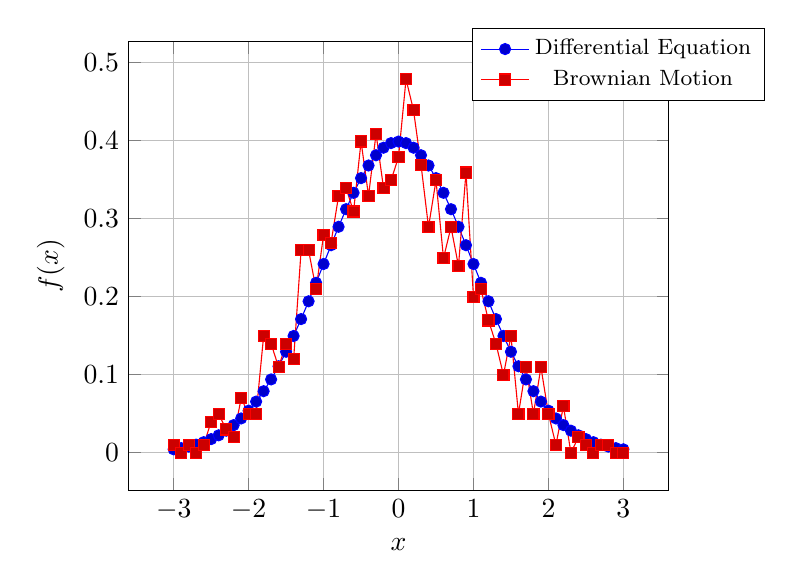
\begin{tikzpicture}
\begin{axis}[legend style={font=\fontsize{8}{4}\selectfont,
        at={(1.18,.95)},
        anchor=east},
    xlabel={$x$},
    ylabel={$f(x)$},
    grid = both,
    legend entries = {Differential Equation, Brownian Motion}
]
\addplot table 
{
  -3.000000000000000   0.004431848411938
  -2.900000000000000   0.005952532419776
  -2.800000000000000   0.007915451582980
  -2.700000000000000   0.010420934814423
  -2.600000000000000   0.013582969233686
  -2.500000000000000   0.017528300493569
  -2.400000000000000   0.022394530294843
  -2.300000000000000   0.028327037741601
  -2.200000000000000   0.035474592846231
  -2.100000000000000   0.043983595980427
  -2.000000000000000   0.053990966513188
  -1.900000000000000   0.065615814774677
  -1.800000000000000   0.078950158300894
  -1.700000000000000   0.094049077376887
  -1.600000000000000   0.110920834679456
  -1.500000000000000   0.129517595665892
  -1.400000000000000   0.149727465635745
  -1.300000000000000   0.171368592047807
  -1.200000000000000   0.194186054983213
  -1.100000000000000   0.217852177032551
  -1.000000000000000   0.241970724519143
  -0.900000000000000   0.266085249898755
  -0.800000000000000   0.289691552761483
  -0.700000000000000   0.312253933366761
  -0.600000000000000   0.333224602891800
  -0.500000000000000   0.352065326764300
  -0.400000000000000   0.368270140303323
  -0.300000000000000   0.381387815460524
  -0.200000000000000   0.391042693975456
  -0.100000000000000   0.396952547477012
                   0   0.398942280401433
   0.100000000000000   0.396952547477012
   0.200000000000000   0.391042693975456
   0.300000000000000   0.381387815460524
   0.400000000000000   0.368270140303323
   0.500000000000000   0.352065326764300
   0.600000000000000   0.333224602891800
   0.700000000000000   0.312253933366761
   0.800000000000000   0.289691552761483
   0.900000000000000   0.266085249898755
   1.000000000000000   0.241970724519143
   1.100000000000000   0.217852177032551
   1.200000000000000   0.194186054983213
   1.300000000000000   0.171368592047807
   1.400000000000000   0.149727465635745
   1.500000000000000   0.129517595665892
   1.600000000000000   0.110920834679456
   1.700000000000000   0.094049077376887
   1.800000000000000   0.078950158300894
   1.900000000000000   0.065615814774677
   2.000000000000000   0.053990966513188
   2.100000000000000   0.043983595980427
   2.200000000000000   0.035474592846231
   2.300000000000000   0.028327037741601
   2.400000000000000   0.022394530294843
   2.500000000000000   0.017528300493569
   2.600000000000000   0.013582969233686
   2.700000000000000   0.010420934814423
   2.800000000000000   0.007915451582980
   2.900000000000000   0.005952532419776
   3.000000000000000   0.004431848411938
   };

   \addplot table
   {


  -3.000000000000000   0.009977212516898
  -2.900000000000000                   0
  -2.800000000000000   0.009977212516898
  -2.700000000000000                   0
  -2.600000000000000   0.009977212516898
  -2.500000000000000   0.039908850067592
  -2.400000000000000   0.049886062584491
  -2.300000000000000   0.029931637550694
  -2.200000000000000   0.019954425033796
  -2.100000000000000   0.069840487618287
  -2.000000000000000   0.049886062584491
  -1.900000000000000   0.049886062584491
  -1.800000000000000   0.149658187753472
  -1.700000000000000   0.139680975236574
  -1.600000000000000   0.109749337685879
  -1.500000000000000   0.139680975236574
  -1.400000000000000   0.119726550202777
  -1.300000000000000   0.259407525439351
  -1.200000000000000   0.259407525439351
  -1.100000000000000   0.209521462854860
  -1.000000000000000   0.279361950473147
  -0.900000000000000   0.269384737956249
  -0.800000000000000   0.329248013057638
  -0.700000000000000   0.339225225574536
  -0.600000000000000   0.309293588023842
  -0.500000000000000   0.399088500675925
  -0.400000000000000   0.329248013057638
  -0.300000000000000   0.409065713192823
  -0.200000000000000   0.339225225574536
  -0.100000000000000   0.349202438091434
                   0   0.379134075642128
   0.100000000000000   0.478906200811110
   0.200000000000000   0.438997350743517
   0.300000000000000   0.369156863125230
   0.400000000000000   0.289339162990045
   0.500000000000000   0.349202438091434
   0.600000000000000   0.249430312922453
   0.700000000000000   0.289339162990045
   0.800000000000000   0.239453100405555
   0.900000000000000   0.359179650608332
   1.000000000000000   0.199544250337962
   1.100000000000000   0.209521462854860
   1.200000000000000   0.169612612787268
   1.300000000000000   0.139680975236574
   1.400000000000000   0.099772125168981
   1.500000000000000   0.149658187753472
   1.600000000000000   0.049886062584491
   1.700000000000000   0.109749337685879
   1.800000000000000   0.049886062584491
   1.900000000000000   0.109749337685879
   2.000000000000000   0.049886062584491
   2.100000000000000   0.009977212516898
   2.200000000000000   0.059863275101389
   2.300000000000000                   0
   2.400000000000000   0.019954425033796
   2.500000000000000   0.009977212516898
   2.600000000000000                   0
   2.700000000000000   0.009977212516898
   2.800000000000000   0.009977212516898
   2.900000000000000                   0
   3.000000000000000                   0
   };
\end{axis}
\end{tikzpicture}
      \caption{Comparing Approaches}\label{fig:1a}
    \end{subfigure}
    \begin{subfigure}[t]{0.48\textwidth}
      \centering
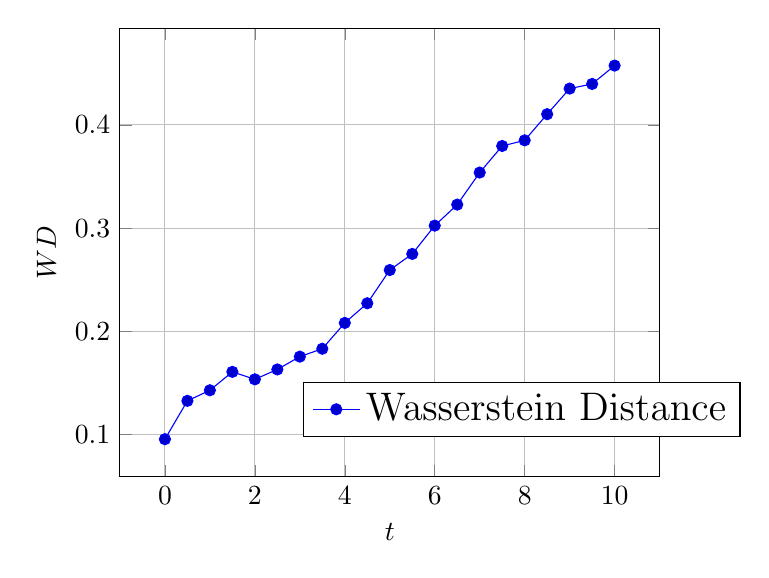
\begin{tikzpicture}
\begin{axis}[legend style={font=\fontsize{15}{5}\selectfont,
        at={(1.15,0.15)},
        anchor=east},
    xlabel={$t$},
    ylabel={$WD$},
    grid = both,
    legend entries = {Wasserstein Distance}
]
\addplot table 
{
                   0   0.095459745805488 
   0.500000000000000   0.132619925678194
   1.000000000000000   0.142863724437454
   1.500000000000000   0.160699344683304
   2.000000000000000   0.153470780324526
   2.500000000000000   0.163047119266944
   3.000000000000000   0.175466336257786
   3.500000000000000   0.183119699694153
   4.000000000000000   0.208128448602138
   4.500000000000000   0.227184509337919
   5.000000000000000   0.259384321795910
   5.500000000000000   0.274999121877102
   6.000000000000000   0.302427937353585
   6.500000000000000   0.322783604585681
   7.000000000000000   0.353867968730460
   7.500000000000000   0.379632470853626
   8.000000000000000   0.385074905130309
   8.500000000000000   0.410417535578750
   9.000000000000000   0.435227246829623
   9.500000000000000   0.439715247612350
  10.000000000000000   0.457522713465409
};

\end{axis}
\end{tikzpicture}
      \caption{Computing the WD}\label{fig:1b}
    \end{subfigure}
  \caption{}\label{fig:1}
\end{figure}
%



The standard approach to modeling complex systems is to use a differential equation. For instance, a biologist interested in studying cancer growth would try to numerically solve
\begin{equation}
\frac{\partial f}{\partial t} = \Big(\frac{\partial^2 f}{\partial x^2} + \frac{\partial^2 f}{\partial y^2}\Big)+ f(1-f).
\label{eq: Macro}
\end{equation}

\noindent While this approach is common, it fails to accurately model the stochastic components of the systems. Dr.\ Motsch and I will examine this same system through the use of Brownian motion. Brownian motion, originally studied by the botanist Robert Brown in the 19th century and popularized by Einstein in the early 20th century, describes motion that behaves in a random way. If an variable's motion is Brownian, its derivative is a normally distributed random variable. By letting $X^m$ denote the particle's location at time $m$, one can use the following equation to compute its future location
\begin{equation}
X^{m+1} = X^{m} + C\textbf{W},
\label{eq: Micro}
\end{equation}


\noindent where $C$ is a constant and $\textbf{W} \sim \mathcal{N}(0, 1).$ Substantial research has been done on theoretical Brownian motion, with little progress on applying these results to complex systems. 

The goal of my research under Dr. Motsch will be to demonstrate that modeling complex systems with Brownian motion, rather than with a differential equation, leads to a more accurate approximation of the underlying dynamics. We will study a reaction-diffusion model in one and two dimensions that can be used to study the growth and death of cancer cells in an organism. In this model, cells are created and destroyed randomly, and so we believe modeling this system using a deterministic differential equation leads to incaccurate solutions. This model on its own is used frequently in academia and industry to understand the behavior of cancer and infectious diseases, and thus an improved solution to this important model will have substantial impact on theoretical and computational biology. To show that the Brownian motion approach is more accutarate, we will compare our results to real-world data obtained from an ASU biology lab. In order to make these comparisons, we will be using a tool in pure mathematics called the Wasserstein Distance (WD), which measures the difference between two data sets. The WD will enable us to quantify the improvement of the Brownian motion approach. 




Dr.\ Motsch and I are well positioned to complete this project. I am an undergraduate student working in applied mathematics who intends to pursue a PhD in statistics. In particular I am interested in applying statistical techniques to solving real-world problems. This past summer I was selected along with three other undergraduates out of over 300 to participate in a research program at San Diego State University. There my advisor and I derived the first method of obtaining convergence behavior for the error in algorithms that one uses when estimating coefficients in the linear regression equation. This project resulted in a publication, and I developed an interest in applying statistical tools to study real-world problems. My role in the project will be to appply statistical techniques to modeling Brownian motion in one and two dimensions and applying numerical techniques to solving the differential equations we'll be using. Dr.\ Motsch received his PhD in applied mathematics with an emphasis in animal cognition and mathematical biology, and works at the intersection of computational math, biology, and statistics. He has overseen undergraduate and graduate theses in flocking behavior, applied statistics, and offers the biological perspective necessary for this project. He has worked previously in the Wasserstein Distance and will provide the background in the WD to apply it to our research.

This project requires an advanced grasp on real analysis, probability theory, and numerical analysis. In order to complete this project successfully, I have enrolled in graduate courses in real analysis,  distribution theory, and stochastic processes. In these courses I will obtain the tools necessary to read papers relating to my project as well as hold informed discussions with Dr. Motsch on our research. I have taken a course on numerical methods with Dr.\ Motsch, and I will use my textbook as a reference during my research. In the Spring I will finish the graduate sequence in real analysis and probability theory.




The Origins Project Scholarship will allow me to focus solely on my research with Dr.\ Motsch, instead of maintaining an on-campus job to pay for college. This will allow me to make faster progress on my research. Having this research experience will also give me the experience necessary to perform well as a graduate student. We believe that the underlying dynamics of stochastic complex systems are different in nature from deterministic models and are therefore not accurately modeled by differential equations. Through this project I seek to better understand these dynamics through statistical modeling. My research with Dr. \ Motsch will demonstrate the possibility of using Brownian motion to model stochastic complex systems, shedding light on the random forces that determine the physical world and on our role as a species in it.


 \newpage


Through this research I will gain the necessary research experience and technical background to succesfully enter into a PhD program in statistics. By publishing our results, I will have an advantage in the application process for graduate school. By conducting this research under Dr.\ Motsch, I'll gain 

This project allows me to apply statistical and numerical techniques to solve tangible problems and provides me with an ideal transition to graduate school. We will be using techniques such as Brownian motion,  approximations of intractable distributions, finite-difference techniques to study differential equations. lysis and graduate distribution theory in the fall to build upon my theoretical foundation.

 Dr.\ Motsch received his PhD in applied mathematics with an emphasis in animal cognition and mathematical biology, and works at the intersection of computational math and biology. He has mentored several undergraduates working in computational biology, flocking patterns, and cell behavior.

The outline of the project is as follows: In September and October, Dr.\ Motsch and I will be submitting a paper to journal that demonstrates that agent-based modeling of complex systems accurately represents the behavior of the complex system using data from \textbf{Motsch, who is this data from?}. In November and December, we will study  and finally in the Spring we will examine. 


As a recipient of the Origins Project Scholarship, I will have the chance to devote myself to my research project, rather than working to pay for college, allowing me and Dr. \ Motsch to make quick progress in our research.  

The Origins Project Scholarship will allow me to focus solely on my research with Dr.\ Motsch, instead of working on campus, allowing for more substantial research progress during the academic year. This will in turn allow me to prepare a stronger graduate school application, 
 The Origins network will provide me and Dr.\ Motsch with an invaluable network of researchers in biology, chemistry and other fields we can speak with, collaborate with, and learn from. This will in turn lead to research that understands the needs of these fields, leading to more helpful and effective results. 


\newpage 
\begin{center}
\textbf{Notes}
\end{center}

 In Figure 1,
the solutions from (\ref{eq: Macro}) and (\ref{eq: Micro}) are plotted.

\textbf{Agent is small, the macro might not be realistic, might not describe. send code and kernel, image I have, and send draft.}

This approach is computationally faster and places no restriction on the physical and temportal discretization, yet there is a problem. There has been little research done that computes the accuracy of this second scheme in relation to the first. Can one trust the answers given by the second approach? \\
The goal of my and Dr. Motsch's research is to prove that the second approach provides an accurate approximation to the system one is considering. We do this using both numerical and pure mathematics. What we show is that researchers in fields as diverse as biology, chemistry, medecine, can faithfully rely on the approximations coming from the second approach. The end result is that researchers in these fields can now solve probems that once seemed inaccesible a few years ago because essentially their computing power has been increased significnatly. 

The answer is that before now, there was very little way to compare the accuracy of the second approach to the first approach. Some ways existed, but they were complicated and required advanced mathematics to fully understand. What Dr. Motsch and I are doing is simplifying the mathematics and deriving simple algorithms that researchers in fields as diverse as biology, chemistry, medecine, etc. can use in their research. What we are doing is allowing these researchers to avoid the complicated mathematics and use the second approach, knowing that this approach is ``close enough'' to the first approach to not be sacrificing accuracy. 

Our first paper is set to be submitted in October. This paper demonstrates that it is possible to use this second approach in approximating biological processes that can be approximated through differential equations. This means that most problems in biology can now be solved through the second approach. Our research indicates that the second approach is 4 times faster than the first approach.

This project lies at the intersection of evolutionary and computational biology, pure mathematics, applied mathematics, and statistics. Dr. Motsch and I are qualified to carry out this project for several reasons. Dr. Motsch received his PhD in applied mathematics with an emphasis in animal cognition and mathematical biology, while I am undergraduate student in pure mathematics intending to obtain a PhD in statistics. Having the opportunity to conduct research as a Origins Scholarship Recipient will allow me to focus solely on my research and finish a second paper with Dr. Motsch. Having three papers on my CV when I apply to PhD programs will be incredibly beneficial. 

The timeline for our project is as follows. In August and September, Dr. Motsch and I are completing work on our first paper, which examines some appliations of the Wasserstein distance to studying the growth of cancer cells. This paper will be submitted at the beginning of October. We will then begin working on a second paper, 


there is a miscmatch, we sometimess need to use micro because it more accurately reflects the underlying truth. agent-based models, complex systems. 

Novel Techniques to Modeling Complex Systems 

Comparison of Agent-based and   
agent-based models for complex systems: 

Modeling Complex Systems: Agent-based Models vs. Macro Models.
Contrasting 


you need large particle for consistency, we need to shift that the 
macro works if number is large enough, but sometimes the system is too small  so that the validity of the macro is questionable.  

it simplifies the computation and allows for more diverse models to be considered. 




two figures: one where it works, one where it doesnt work., the one where that it doesnt work, in some sort of experimental data, we'll hold off for now. we want to use opacity, level curves, difference both macro and micro. 

open question: compare micro vs. macro, sometimes one doesnt work when n isnt large enough. We need statistics to study the behavior of agent-based when the macro is not enough.  







To solve such an equation, one discretizes the physical space (corresponding to the $x$ and $y$ variables) and the temporal space (corresponding to the $t$ variable). This approach requires the ratio $\frac{\Delta t}{\Delta x^2}$ to be very small in order for the solution to be accurate. This results in a computationally expensive problem. Furthermore, as the physical space gets larger, the computational time required increases exponentially. For problems of even moderate size, this approach is therefore impracticle.\\ 


Many biological processes can be 

As our computing power inceases, questions that once seemed impossible to analyze become accessible. Faster computation has faciliatated new discoveries in computer science, physics, and chemistry, but nowhere are these discoveries more important to our understanding of the physical world than in biology. Biological processes, such as the growth of cancer, the spread of disease, or the evolution of a species, are at the forefront of modern science, and understanding these processes is critical to understanding our place in the universe. Working under Dr. S\'{e}bastien Motsch, my Origins Project work will focus on deriving faster, more accurate approaches to analyzing complex dynamical systems.



\end{document}  

                  0   0.095459745805488 
   0.100000000000000   0.103038153835043
   0.200000000000000   0.122390116625128
   0.300000000000000   0.132687398532943
   0.400000000000000   0.141253013593047
   0.500000000000000   0.132619925678194
   0.600000000000000   0.132080641788240
   0.700000000000000   0.126684962315643
   0.800000000000000   0.126916579284260
   0.900000000000000   0.130572856315571
   1.000000000000000   0.142863724437454
   1.100000000000000   0.151314041878340
   1.200000000000000   0.157724124185497
   1.300000000000000   0.157487782560854
   1.400000000000000   0.150699563747470
   1.500000000000000   0.160699344683304
   1.600000000000000   0.138550211752228
   1.700000000000000   0.141804472307241
   1.800000000000000   0.139818367972234
   1.900000000000000   0.146181574882163
   2.000000000000000   0.153470780324526
   2.100000000000000   0.157789500372874
   2.200000000000000   0.164623391004034
   2.300000000000000   0.174651856775786
   2.400000000000000   0.165106253910355
   2.500000000000000   0.163047119266944
   2.600000000000000   0.165371933076515
   2.700000000000000   0.168312824055832
   2.800000000000000   0.163027901066160
   2.900000000000000   0.165021445928958
   3.000000000000000   0.175466336257786
   3.100000000000000   0.169441333113976
   3.200000000000000   0.167736362245388
   3.300000000000000   0.174500263853999
   3.400000000000000   0.176807926512032
   3.500000000000000   0.183119699694153
   3.600000000000000   0.186685386248164
   3.700000000000000   0.190381205104428
   3.800000000000000   0.196700741959594
   3.900000000000000   0.199003478468923
   4.000000000000000   0.208128448602138
   4.100000000000001   0.212927381498538
   4.200000000000000   0.216035775125143
   4.300000000000000   0.216309196519999
   4.400000000000000   0.226192482106804
   4.500000000000000   0.227184509337919
   4.600000000000001   0.232672773797666
   4.700000000000000   0.244151932180668
   4.800000000000001   0.245019748714593
   4.900000000000000   0.247101950208486
   5.000000000000000   0.259384321795910
   5.100000000000000   0.262244593436841
   5.199999999999999   0.263736387029788
   5.300000000000000   0.271223425250633
   5.399999999999999   0.269171050595840
   5.500000000000000   0.274999121877102
   5.600000000000000   0.280189726935880
   5.700000000000000   0.278080380840482
   5.800000000000000   0.284123569488352
   5.899999999999999   0.293092319792321
   6.000000000000000   0.302427937353585
   6.100000000000000   0.304988685584145
   6.199999999999999   0.310875304199478
   6.300000000000000   0.309492394889520
   6.400000000000000   0.316683383435123
   6.500000000000000   0.322783604585681
   6.600000000000000   0.327349943001851
   6.699999999999999   0.337347746399912
   6.800000000000000   0.344809074579488
   6.900000000000000   0.350911235743597
   7.000000000000000   0.353867968730460
   7.100000000000000   0.359376409561387
   7.199999999999999   0.367885437481766
   7.300000000000000   0.372205234477801
   7.400000000000000   0.376966998227070
   7.500000000000000   0.379632470853626
   7.600000000000000   0.382266518732972
   7.699999999999999   0.379917749569585
   7.800000000000000   0.378863138190330
   7.900000000000000   0.386603623292818
   8.000000000000000   0.385074905130309
   8.100000000000000   0.392721329717624
   8.199999999999999   0.395608310610736
   8.300000000000001   0.399023272131075
   8.400000000000000   0.406569688035700
   8.500000000000000   0.410417535578750
   8.600000000000000   0.419335508882418
   8.699999999999999   0.423990982698414
   8.800000000000001   0.424340729563118
   8.900000000000000   0.423686816264073
   9.000000000000000   0.435227246829623
   9.100000000000000   0.435876153253802
   9.199999999999999   0.428210125789563
   9.300000000000001   0.432099295650654
   9.400000000000000   0.438695163168372
   9.500000000000000   0.439715247612350
   9.600000000000000   0.442966420891081
   9.699999999999999   0.444992993534448
   9.800000000000001   0.453284818856704
   9.900000000000000   0.459222943838312
  10.000000000000000   0.457522713465409

  Cancer researchers rely on accurate approximations of the cell's behavior to derive more effective treatments, and


What we dont understand in biology can be modeled by stochastic components, and we believe that this research will lead to breakthroughs in fields of biology 

-there is more going on than what is reflected in the deterministic. 
- pde occurs becaose of LLN, but here we are in the case of when we are not in this case.  




 has two main goals. The first goal is to more accurately model random complex systems using Brownian motion. By using tools in real analysis, probability theory, and numerical methods, our work will seek to show that Brownian motion can better model complex systems than the current approach. The second goal of our project is to quantify the improvement our approach has over the current approach. 


In order to compare the accuracy of our approach to the accuracy of the traditional approach to modeling complex system, we need a way to quantify the difference between our solutions. In the past few years a new tools was proposed.  much research has been done on the Wasserstein Distance, a tool in pure mathematics that quantifies the difference between functions. Entirely theoretical, we want to show that this distance can be used quite effectively to quantify the difference between the Brownian motion approach and the differential equation approach. The second goal of this project is to take a tool that has been up until now a purely theoretical tool and show that it can be used to effectively quantify the difference in approaches to modeling stochastic complex systems.




